\section{Nessie}
\label{sec:Nessie}

The NEtwork Scalable Service Interface, or Nessie, is a framework for developing
parallel client-server data services for large-scale HPC
systems~\cite{lofstead:2011:nessie-staging,oldfield:lwfs-data-movement,oldfield:2012:uGNI}. 

Nessie was originally developed out of necessity for the Lightweight File
Systems (LWFS) project~\cite{oldfield:lwfs}, a joint effort between researchers
at Sandia National Laboratories and the University of New Mexico. The LWFS
project followed the basic philosophy of ``simplicity enables scalability'',
the foundation of earlier work on lightweight operating system kernels at
Sandia~\cite{riesen:ccpe-lwk}. The LWFS approach was to provide a core set of
fundamental capabilities for security, data movement, and storage and afford
extensibility through the development of additional services. For example,
systems that require data consistency and persistence might create services for
transactional semantics and naming to satisfy these requirements. The Nessie
framework was designed to be the vehicle to enable the rapid development and 
deployment of such services.  


Although Nessie was originally designed for I/O and system services, it is also
useful for development of application-specific data services.  For example, 
we developed services for staging checkpoint
data~\cite{oldfield:ft-ldrd-tr,reiss:checkpoint-proxy,oldfield:modeling_checkpoints},
HPC database integration~\cite{oldfield:sql-proxy}, interactive
visualization~\cite{oldfield:multilingual-siam}, network traffic analysis, and 
most recently CTH \intransit analysis~\cite{moreland:2011:in-transit}.  A recent
paper describes these services in detail~\cite{lofstead:2013:data-staging}.


This section includes a brief description of the Nessie architecture and APIs followed
by a more detailed description of the \intransit service for CTH analysis using 
ParaView.  


\subsection{Nessie Architecture}

Because Nessie was originally designed for I/O systems, it includes a number of
features that address scalability, efficient data movement, and support for
heterogeneous architectures. Features of particular note include 1)~using
asynchronous methods for most of the interface to prevent client blocking while
the service processes a request; 2)~using a server-directed approach to
efficiently manage network bandwidth between the client and servers; 3)~using
separate channels for control and data traffic; and 4)~using XDR encoding for
the control messages (i.e., requests and results) to support heterogeneous
systems of compute and service nodes.

A Nessie service consists of one or more processes that execute as a serial
or parallel job on the compute nodes or service nodes of an HPC system. We have
demonstrated Nessie services on the Cray XT and XE systems at Sandia National
Laboratories (SNL) and Oak Ridge National , the Cray XT4/5 systems at Oak Ridge National Laboratory,
and a large InfiniBand
cluster at SNL. The Nessie RPC layer has direct support of Cray's SeaStar
interconnect~\cite{brightwell:2006:seastar}, through the Portals
API~\cite{brightwell:2002:portals3}; Cray's Gemini
interconnect~\cite{alverson:2010:gemini}; and
InfiniBand~\cite{infiniband:specification}.  

\subsubsection{Nessie API}

The Nessie API follows a remote procedure call (RPC) model, where the client
(i.e., the scientific application) tells the server(s) to execute a function on
its behalf.  Nessie relies on client and server stub functions to encode/decode
(i.e., marshal) procedure call parameters to/from a machine-independent format.
This approach is portable because it allows access to services on heterogeneous
systems, but it is not efficient for I/O requests that contain raw buffers that
do not need encoding. It also employs a `push' model for data transport that
puts tremendous stress on servers when the requests are large and unexpected,
as is the case for most I/O requests.


To address the issue of efficient transport for bulk data, Nessie uses separate
communication channels for control and data messages. In this model, a ``control''
message, also known as a request, is typically small. It identifies the
operation to perform, where to get arguments, the structure of the arguments,
and perhaps the data itself (if the data is small enough to fit in the
fixed-sized request).  In contrast, a data message is typically large and
consists of ``raw'' bytes that, in most cases, do not need to be
encoded/decoded by the server. For example,
Figure~\ref{fig:nssi-movement-protocol} shows the transport protocol for an
\intransit service that performs analysis of simulation data.

\begin{figure}
\begin{centering}
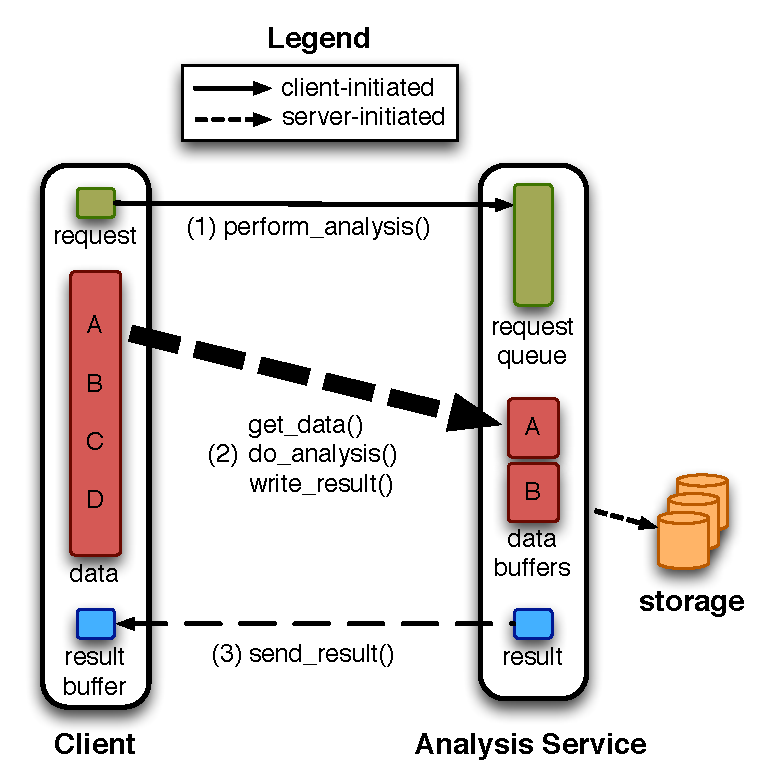
\includegraphics[scale=0.6]{figures/ServerDirected}
\caption[Nessie transport protocol]{Conceptual protocol for Nessie service doing analysis.  
The server fetches bulk data through
RDMA commands until it has satisfied the request.  After completing the
data transfers, the server processes the data, writes analysis results
to disk, then sends a small ``result'' back to the client
indicating success or failure of the operation.}
\label{fig:nssi-movement-protocol}
\end{centering}
\end{figure}

The Nessie client uses the RPC-like interface to push control messages to the
servers, but the Nessie server uses a different, one-sided API to push or pull
data to/from the client. This protocol allows interactions with heterogeneous
servers and benefits from allowing the server to control the transport of
bulk data~\cite{kotz:bdiskdir,seamons:panda}. The server can thus manage large
volumes of requests with minimal resource requirements. Furthermore, since
servers are expected to be a critical bottleneck in the system, a server
directed approach affords the server optimizing request processing for
efficient use of underlying network and storage devices -- for example,
re-ordering requests to a storage device~\cite{kotz:bdiskdir}.

While it is not strictly necessary on systems that have homogenous clients and servers, we 
use XDR encoding to provide portable serialization of arguments for the request arguments. 
This was a design decision made early in the project that allow the client to
send arbitrary C-like data structures to the server with minimal development effort.  At 
the time, we were implementing file services for a system where the service nodes were
a different architecture (and had different endienness) than the compute nodes.  In this 
case, byte-swaps were necessary for the control structures.  Since
\emph{rpcgen}, the function that generates the serialization code is pervasive in Unix
environments and has been in use for more than a decade, it was the logical choice for 
argument marshaling.  

\subsubsection{NNTI API}

The Nessie Network Transport Interface (NNTI) provides a portable, lightweight,
interface for RDMA operations on HPC platforms.  Our current
implementation includes support for the Cray Seastar, InfiniBand,
Cray Gemini, and IBM DCMF interconnects.  The APIs include commands
to open and close the interface, connect and disconnect to a peer,
register and deregister memory buffers, and finally asynchronously transport
(through put, get, and wait commands) bulk data. 

\begin{figure}
\begin{centering}
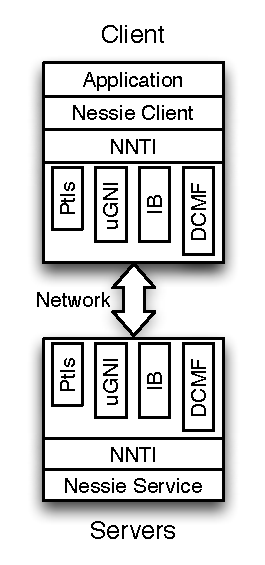
\includegraphics{figures/NSSISoftwareStack}
\par\end{centering}
\caption{Software stack for applications using the Nessie and NNTI libraries.}
\end{figure}


Figure~\ref{fig:nssi-software-stack} illustrates the software stack for applications 
using Nessie and NTTI. The NNTI library sits below the Nessie RPC library to
enable portability across HPC interconnects.  In addition to the Nessie
library, NNTI is also used by the
ADIOS/DataStager~\cite{abbasi:2010:datastager} to provide the same level of
portability and performance.  We are also discussing NNTI as the lowest-layer
network transport for the Sirocco parallel file system, another ASC project at
SNL.

\subsubsection{CommSplitter API}

The CommSplitter library was designed to overcome a security model limitation in
the Gemini interconnect.  On current Gemini systems, user-space applications
are not allowed to communicate, even if both applications are owned by the same
user.  We requested this feature and at the time of this writing, Cray is
addressing this issue to better support data services in future versions of
Gemini.  In the mean time, we overcame that limitation by launching our jobs in
Multiple Program, Multiple Data (MPMD) mode.  MPMD mode enables a set of
applications to execute concurrently, sharing a single MPI Communicator.   The
problem with this approach is that legacy applications were not designed to
share a communicator with other applications.  In fact, most HPC codes assume
they have exclusive use of the \texttt{MPI\_COMM\_WORLD} communicator.  When
this is not the case, a global barrier, such as an \texttt{MPI\_Barrier}
function will hang because the other applications did not call the
\texttt{MPI\_Barrier} function. 

To address this issue, we developed the CommSplitter library to allow
applications to run in MPMD mode while still maintaining exclusive access to a 
virtual \texttt{MPI\_COMM\_WORLD} global communicator.  

The CommSplitter library identifies the processes that belong to each
application, then ``split'' the real \texttt{MPI\_COMM\_WORLD} into separate
communicators.   The library then uses the MPI profiling interface to intercept
MPI operations, enforcing the appropriate use of communicators for
collective operations.

No changes are required to the application source code to enable this
functionality.  The user simply links the CommSplitter library to the executable
before launching the job.  The library has no effect on applications that are
not run in MPMD mode. 



\subsection{CTH \intransit analysis}

In this milestone, we used Nessie to construct an \intransit CTH analysis 
service.  The analysis service exists as its own parallel job 
that communicates with a parallel CTH job using the Nessie APIs.  
The \intransit CTH analysis library is a drop-in replacement
for the PVSPY library~\cite{moreland:2010:coprocessing-milestone} used for
\insitu analysis.  This makes comparing \insitu and \intransit approaches
extremely convenient since it only requires the user to link a different
library when compiling CTH.  Instead of executing the analysis on the 
same compute nodes of the CTH application (as the \insitu library does), the
\intransit library marshals requests, sends data to the analysis service, and
performs all the analysis on the separate application.
Figure~\ref{fig:cth-service} illustrates this process for analysis that does
fragment detection. 

\begin{figure*}
\begin{centering}
\subfloat[\Insitu analysis]{
  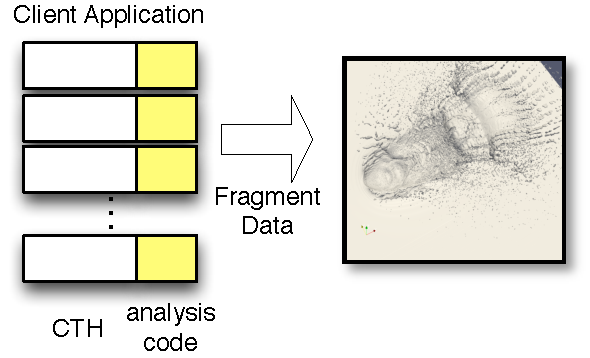
\includegraphics[scale=0.55]{figures/cth-in-situ}
  \label{fig:cth-in-situ}
}
\subfloat[\Intransit analysis]{
  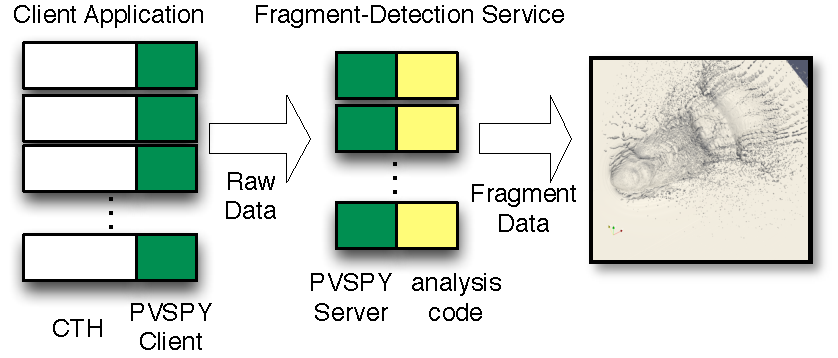
\includegraphics[scale=0.55]{figures/cth-in-transit}
  \label{fig:cth-in-transit}
}
\caption[\Insitu and \Intransit Analysis]{Comparison of \insitu (a) and \intransit (b)
fragment detection for the CTH shock physics code.}
\label{fig:cth-service}
\end{centering}
\end{figure*}

% There are a couple of trade-offs to consider when deciding whether to perform
% the analysis \intransit or \insitu.  First, the \intransit approach allows
% fragment detection to execute in parallel with CTH, unlike the \insitu approach
% that requires CTH to wait for the analysis to complete.  If the time to execute
% the analysis code is substantially larger than the time to transfer the raw data
% to the service, there is a performance advantage to using the \intransit
% approach.

% A second consideration is library scalability.  While significant effort has
% gone into making the CTH code scale to extremely large core counts, not as much
% effort has gone into scalability of the analysis code.  For example, the
% ParaView coProcessing libraries have not successfully run on more than 32
% thousand cores.  Linking CTH to ParaView for \insitu analysis also limits the
% scalability of the CTH run.  In contrast, the data service will likely use
% a much smaller number of cores, putting no limitation on the scale of CTH. 

% Another often overlooked consideration is the memory required to link a large
% analysis library into a production scientific code.  In the \insitu case, CTH
% has to link ParaView.  Since many HPC systems do not efficiently support dynamic
% libraries\footnote{Support for dynamic libraries is currently being evaluated
% for the Cray XE6.}, the entire static ParaView library has to be linked. On the
% Cray XE6, the \insitu binary for CTH is 330 MiB, where the \intransit binary for CTH is 30
% MiB.  That is a substantial difference, especially on systems that are memory
% limited -- as is the case for most multi-core HPC platforms.


For efficiency reasons, the \intransit PVSPY client implementation does not
simply forward all the functions to the service.  In many cases, the client
maintains metadata to avoid unnecessary data transfers.  For example, the PVSPY
API includes ``setup'' functions for initializing data structures, assigning
cell and material field names, and setting cell and material fields pointers.
Not all of these functions require an immediate interaction with the data
service.  In fact, the only operations that require bulk data transport are
the operations that synchronize the metadata and the data between the client 
and the server.  These operations occur just before a \emph{pvspy\_viz} operation
that initiates the ParaView coProcessing on the remote service. 

The \insitu version of PVSPY has the notion of a ``CTH source'' that allows the
analysis code to work directly on the memory of the CTH application without
making any copies.   Since the \intransit service does not have access to the
physical memory of the CTH application, we created a virtual CTH source on the
server that emulates the data structures on the CTH application.  That allows
the service to use use the same PVSPY library that the client uses in the \insitu
analysis.  

With the exception of the operations to transfer metadata and data to the analysis
service, all remote operations are asynchronous, allowing the analysis on the 
service to execute in parallel with computation on the CTH application.  If one
remote visualization operation is not complete by the time CTH is ready to do another
visualization operation, CTH has to wait. 


\subsection{Related Efforts}

There are a number of efforts to develop technologies for staging data or 
providing data services that are related to, and in some cases derived from,
Nessie.  The two primary competitors of Nessie include the data-staging
portions of the ADIOS library from ORNL, and the Glean library from Argonne
National Laboratory. 

The Adaptable IO System (Adios) is an I/O library that separates the I/O
interface from the underlying I/O operations.  Using XML configuration 
files, the user can specify, at runtime, the methods used to perform I/O.
For example, MPI-IO, POSIX-IO, netCDF, or their own BP method are all options
the use can select.  ADIOS also includes methods data transport that allow
the staging and processing of data in the same way as Nessie.  This staging
technology, called DataTap~\cite{datatap2009cluster} and
DataStager~\cite{abbasi:2010:datastager} derive from early work on Nessie as
part of a joint collaboration between GA Tech, SNL, and ORNL.  More recent
versions of DataStager are also using the NNTI API to provide portable 
RDMA transport. 

The DataSpaces~\cite{docan:2010:dataspaces} project uses the memory on
data-staging nodes as a scratch space for communicating and sharing 
data among multiple applications.  This work is closely aligned with the 
ADOIS efforts at ORNL.  The primary focus is to use asynchronous IO to
move data into a staging area and then having a
different application retrieve data at a later time.

A recent effort called Glean~\cite{vishwanath:2011:glean} from Argonne is a
start towards both accelerating IO performance and integrating functionality,
such as analysis routines, at the right place transparently. It is very similar
to PreDatA, but extends the location of operations to potentially beyond the
current machine.

Most of the related efforts focus primarily on the I/O benefits of data-staging, but
have not put a tremendous effort into complex analysis. The majority of the analyis
codes perform relatively simple statistics and/or visualization.  With Nessie, and 
this effort in particular, we treat the service as a complex parallel application
that includes all the synchronization, communication, and scaling issues inherent in HPC 
parallel applications.  These issues require a level of detail and performance 
tuning that is lacking in other efforts.  

A second distinction between our approach and related work is a general 
philosophy on supporting APIs.  While the other approaches, like ADIOS,
provide a unified I/O API, our approach is to provide \intransit
implementations of commonly used APIs so the code does not have to change the
source code.  In this milestone, we implemented an \intransit version of
the pvspy API, the same API used to perform the \insitu experiments.  It was
this approach that made comparison between the \insitu and \intransit
approaches so easy to perform.

\subsection{Nessie Availability}

The Nessie software is available, open source, as part
of the Trilinos I/O Support Package~\cite{oldfield:2012:trios-journal}.
The package includes the NNTI, Nessie, CommSplitter libraries as well
as a collection of CMake macros and other tools for constructing 
application-specific data services.


